\documentclass[aspectratio=169]{beamer}

\usepackage{nth}
\usepackage{polyglossia}
\usepackage{tikz}
\usepackage{graphbox}
\usetikzlibrary{shapes, arrows, matrix, fit}

\setdefaultlanguage[variant=british]{english}

\setcounter{tocdepth}{1}

\let\oldsection\section
\renewcommand{\section}[1]{
	\oldsection{#1}	
	\subsection{}
}

\newenvironment{myframe}[1][t]{\begin{frame}[#1]{\secname}{\subsecname}}{\end{frame}}

\usetheme{cranfielduniversity}

\author[Miguel Marques]{Miguel Marques}
\supervisor{Supervisor: Dr. Peter Sherar}
\course{MSc in Computational and Software Techniques in Engineering \\ Digital Signal and Image Processing}

\title{Web Based Terrain Modeller}
\date{22\textsuperscript{nd} July 2016}

\begin{document}
	
	\begin{frame}
		\titlepage
	\end{frame}
	
	\begin{frame}[t]{Outline}
	{
		\renewcommand{\baselinestretch}{1.5}
		\begin{columns}[t]
			\begin{column}{\textwidth}
				\tableofcontents
			\end{column}
		\end{columns}	
	}
	\end{frame}
	
	\section{Problem}
	
	\begin{myframe}
		\vspace{-0.75cm}
		\begin{block}{Functional Requirements}
			\begin{itemize}
				\item Procedurally generate detailed terrains
				\item Use a CAD surface as a base
			\end{itemize}
		\end{block}
		\begin{block}{Technical Requirements}
			\begin{itemize}
				\item Web-based
				\item Based on fractal geometry
			\end{itemize}
		\end{block}
		\begin{block}{Additional Requirements}
			\begin{itemize}
				\item Real-time editing
			\end{itemize}
		\end{block}
	\end{myframe}
	
	\section{Relevant Background}
	
	\subsection{Fractals}
	
	\begin{myframe}
		\begin{columns}[t]
			\begin{column}[t]{0.6\linewidth}
				\centering
				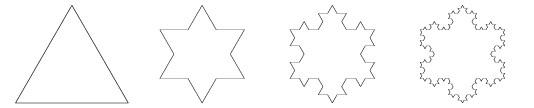
\includegraphics[align=t, width=0.7\linewidth]{images/background/fractals/koch} \\[0.5em]
				\tiny\textit{in Weisstein, Eric W. "Koch Snowflake." From MathWorld -- A Wolfram Web Resource. http://mathworld.wolfram.com/KochSnowflake.html} \\ [1.5em]
				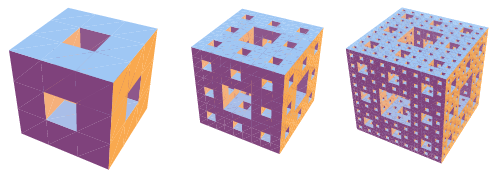
\includegraphics[align=t, width=0.7\linewidth]{images/background/fractals/sponge} \\[0.5em]
				\tiny\textit{in Weisstein, Eric W. "Menger Sponge." From MathWorld -- A Wolfram Web Resource. http://mathworld.wolfram.com/MengerSponge.html}
			\end{column}
		\end{columns}
		
		
	\end{myframe}
	
	\subsection{Fractional Brownian Motion (fBm)}
	
	\begin{myframe}
		\begin{columns}[t]
			\begin{column}[t]{0.4\linewidth}
				$D_f = D_E + 1 - H$ \\[1em]
				\scriptsize{
					\hspace{-1em}
					\begin{tabular}{p{0.5em}l}
						$D_f$ & Fractal dimension \\
						$D_E$ & Euclidean dimension \\
						$H$ & Hurst Exponent
					\end{tabular}
				}
			\end{column}
			\begin{column}[t]{0.5\linewidth} 
				\begin{tabular}[t]{rl}
					\tiny\parbox[c]{5em}{$H = 0.0$} & 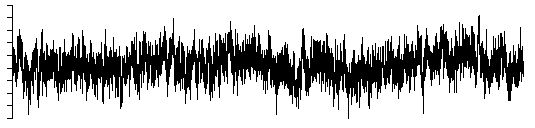
\includegraphics[align=c,width=0.775\linewidth]{images/background/brownian/noise10} \\ [1.5em]
					\tiny\parbox[c]{5em}{$H = 0.5$} & 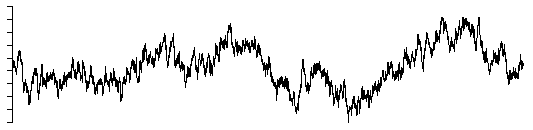
\includegraphics[align=c,width=0.775\linewidth]{images/background/brownian/noise20} \\ [1.5em]
					\tiny\parbox[c]{5em}{$H = 1.0$} & 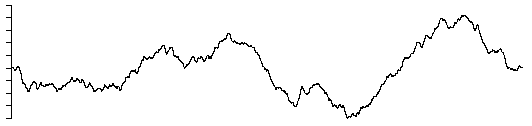
\includegraphics[align=c,width=0.775\linewidth]{images/background/brownian/noise30}
				\end{tabular} \\[0.5em]
				\begin{flushright}\tiny\textit{in http://paulbourke.net/fractals/noise/}\hspace{3em}\end{flushright}
			\end{column}
		\end{columns}
	\end{myframe}
	
	\subsection{Terrain Representation}
	
	\begin{myframe}
		\begin{columns}[T]
			\begin{column}{0.45 \linewidth}
				\textbf{Height Map}
				\begin{itemize}
					\item Two dimensional array
					\item Each position saves an altitude value
					\item Can be saved as a grayscale image
				\end{itemize}
			\end{column}
			\begin{column}{0.45 \linewidth}
				\vspace{-0.5cm}
				\begin{figure}[c]
					\centering
					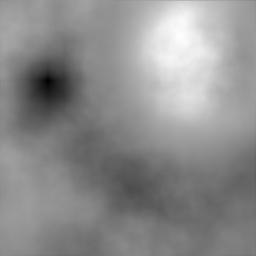
\includegraphics[width=0.7\linewidth]{images/background/representation/heightmap} \\
					\scriptsize\textit{Example of height map}
				\end{figure}
			\end{column}
		\end{columns}
	\end{myframe}
	
	%	\begin{myframe}
	%		\begin{columns}[T]
	%			\begin{column}{0.45 \linewidth}
	%				\textbf{Triangulated Irregular Network}
	%				\begin{itemize}
	%					\item List of 3D vertices
	%					\item Resembles a generic 3D model representation					
	%					\item Supports overhangs
	%				\end{itemize}
	%			\end{column}
	%			\begin{column}{0.45 \linewidth}
	%				\begin{figure}[c]
	%					\centering
	%					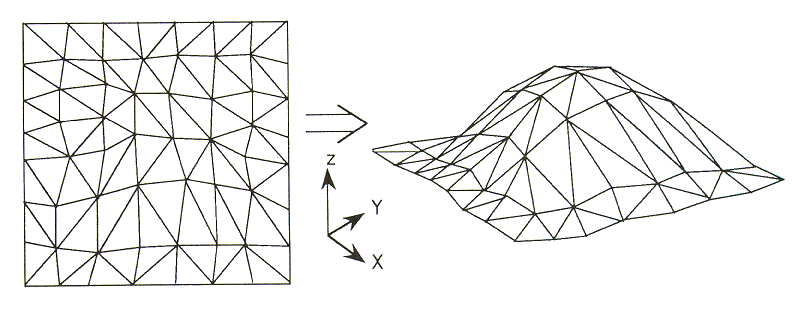
\includegraphics[height=7.5em]{images/background/representation/tin} \\
	%					\parbox{1.1\linewidth}{\tiny\textit{in http://wtlab.iis.u-tokyo.ac.jp/~wataru/lecture/rsgis/rsnote/cp6/cp6-10.htm}}
	%				\end{figure}
	%			\end{column}
	%		\end{columns}
	%	\end{myframe}
	
	\begin{myframe}
		\begin{columns}[T]
			\begin{column}{0.45 \linewidth}
				\textbf{Regular Grid}
				\begin{itemize}
					\item Wireframe processing
					\item Rendering
				\end{itemize}
			\end{column}
			\begin{column}{0.45 \linewidth}
				\begin{figure}[c]
					\hspace{-0.95cm}
					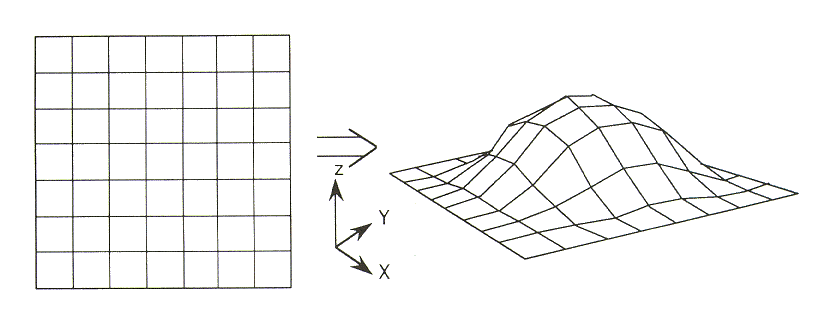
\includegraphics[height=7.6em]{images/background/representation/grid} \\
					\hspace{-0.65cm}
					\parbox{1.05\linewidth}{\tiny\textit{in http://wtlab.iis.u-tokyo.ac.jp/~wataru/lecture/rsgis/rsnote/cp6/cp6-10.htm}}
				\end{figure}
			\end{column}
		\end{columns}
	\end{myframe}
	
	\subsection{Terrain Generation Methods}
	
	\begin{myframe}
		\begin{columns}[T]
			\begin{column}{0.45\linewidth}
				\begin{itemize}
					\item Poisson Faulting
					\item Subdivision Methods
					\item Fourier Filtering
					\item Noise Synthesis
				\end{itemize}
			\end{column}
			
			\begin{column}{0.5\linewidth}
			\end{column}
		\end{columns}
	\end{myframe}
	
	\begin{myframe}
		\begin{columns}[T]
			\begin{column}{0.45\linewidth}
				\begin{itemize}
					\item \textbf{Poisson Faulting}
					\item Subdivision Methods
					\item Fourier Filtering
					\item Noise Synthesis
				\end{itemize}
			\end{column}
			
			\begin{column}{0.5\linewidth}
				\vspace{-1.5em}
				\begin{tabular}{lr}
					
\includegraphics[width=0.35\linewidth]{images/background/generation/plane10} &
					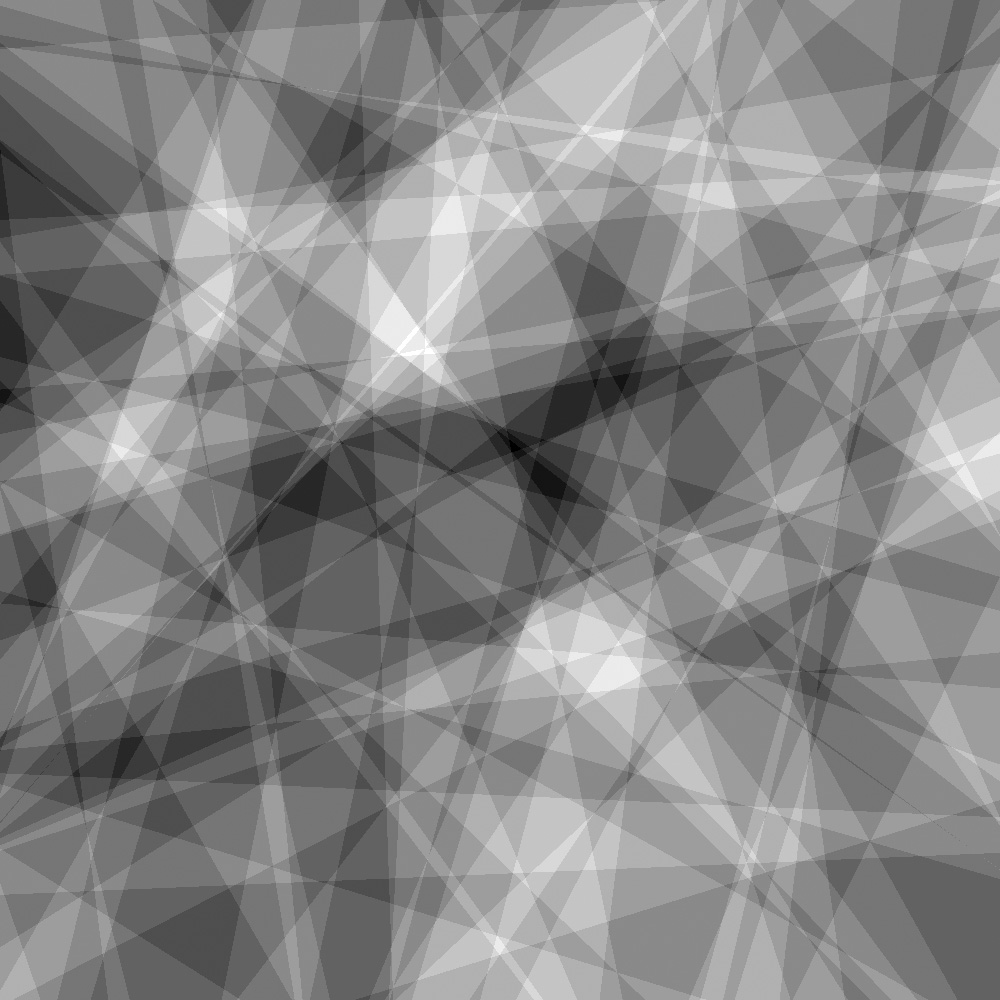
\includegraphics[width=0.35\linewidth]{images/background/generation/plane100} \\
					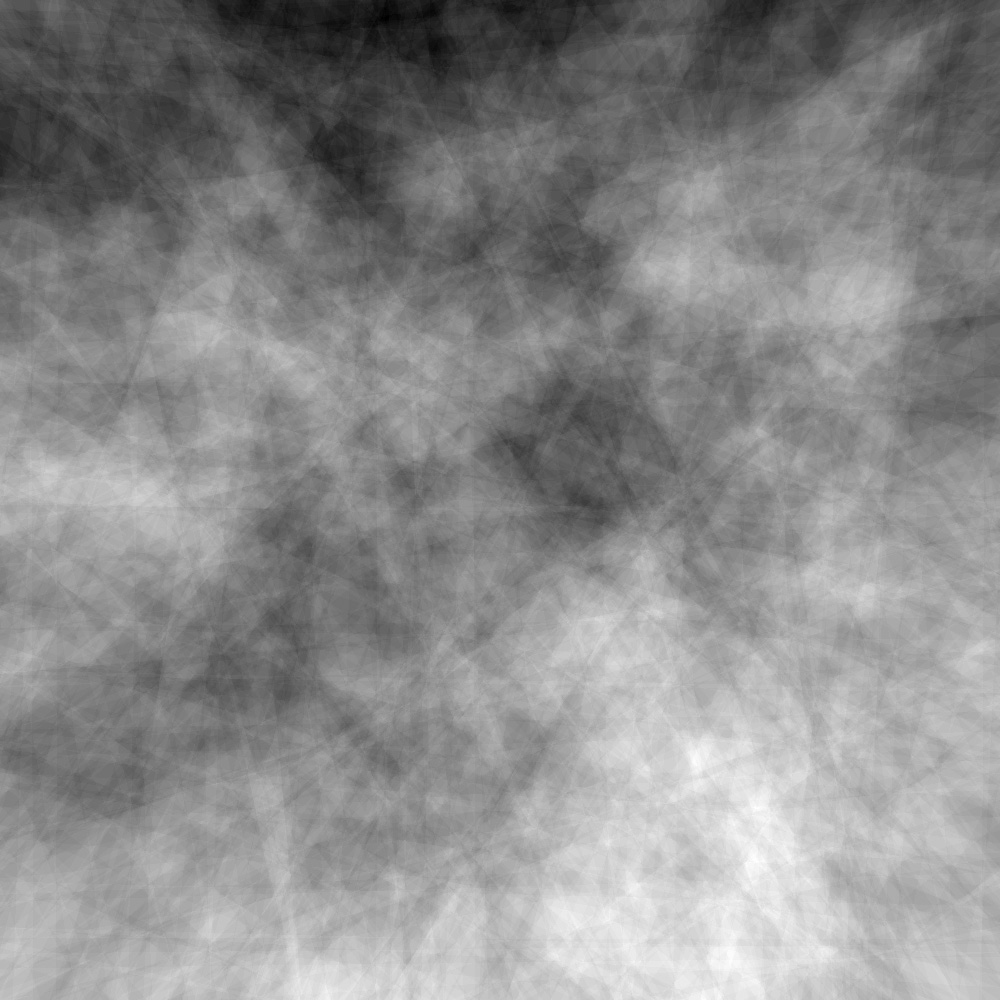
\includegraphics[width=0.35\linewidth]{images/background/generation/plane1000} &
					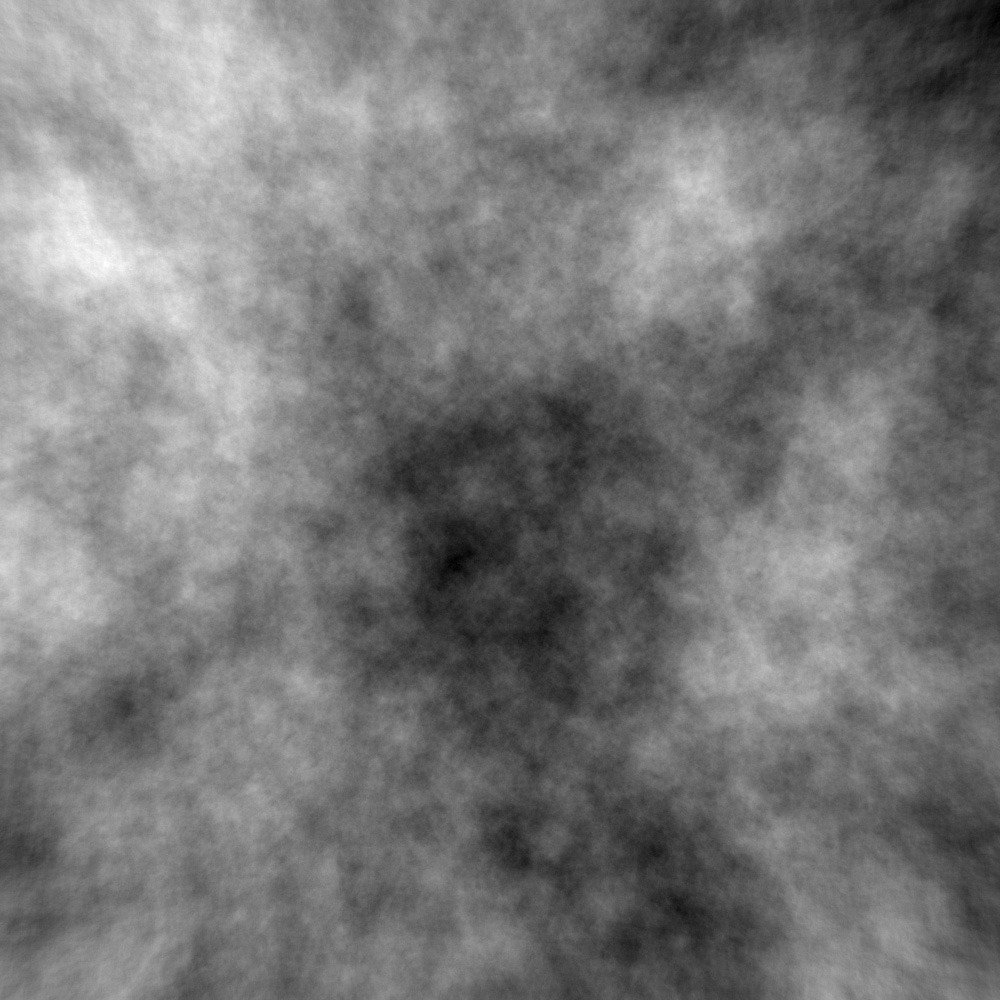
\includegraphics[width=0.35\linewidth]{images/background/generation/plane100000} \\
					\multicolumn{2}{r}{\tiny\textit{in http://paulbourke.net/fractals/noise/}}
				\end{tabular}
			\end{column}
		\end{columns}
	\end{myframe}
	
	\begin{myframe}
		
		\begin{columns}[T]
			\begin{column}{0.45\linewidth}
				\begin{itemize}
					\item Poisson Faulting
					\item \textbf{Subdivision Methods}
					\item Fourier Filtering
					\item Noise Synthesis
				\end{itemize}
			\end{column}
			
			\begin{column}{0.5\linewidth}
				\begin{tabular}{r}
					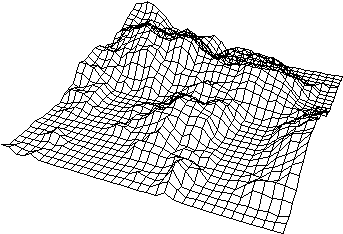
\includegraphics[width=0.7\linewidth]{images/background/generation/subdivision} \\
					\tiny\textit{in http://paulbourke.net/fractals/noise/}
				\end{tabular}
			\end{column}
		\end{columns}
	\end{myframe}
	
	\begin{myframe}
		\begin{columns}[T]
			\begin{column}{0.45\linewidth}
				\begin{itemize}
					\item Poisson Faulting
					\item Subdivision Methods
					\item \textbf{Fourier Filtering}
					\item Noise Synthesis
				\end{itemize}
			\end{column}
			
			\begin{column}{0.5\linewidth}
				$\beta = 1 + 2 H \Leftrightarrow H = \frac{\beta - 1}{2}$ \\[1em]
				$D_f = D_E + 1 - H = D_E + \frac{3-\beta}{2}$ \\[1.5em]
				\scriptsize{
					\hspace{-1em}
					\begin{tabular}{p{0.5em}l}
						$D_f$ & Fractal dimension \\
						$D_E$ & Euclidean dimension \\
						$H$ & Hurst Exponent \\
						$\beta$ & Filter Power
					\end{tabular}
				}
			\end{column}
		\end{columns}
	\end{myframe}
	
	\begin{myframe}
		\begin{columns}[T]
			\begin{column}{0.45\linewidth}
				\begin{itemize}
					\item Poisson Faulting
					\item Subdivision Methods
					\item Fourier Filtering
					\item \textbf{Noise Synthesis}
				\end{itemize}
			\end{column}
			
			\begin{column}{0.5\linewidth}
				\vspace{-1.5em}
				\begin{tabular}{lr}
					
\includegraphics[width=0.35\linewidth]{images/background/generation/pnoise-1} &
					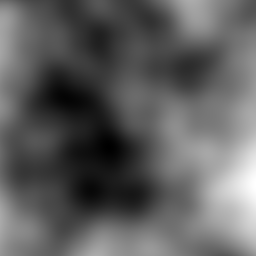
\includegraphics[width=0.35\linewidth]{images/background/generation/pnoise-2} \\
					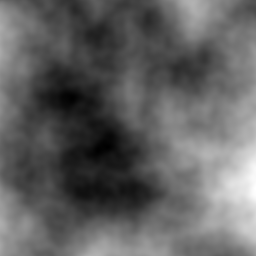
\includegraphics[width=0.35\linewidth]{images/background/generation/pnoise-4} &
					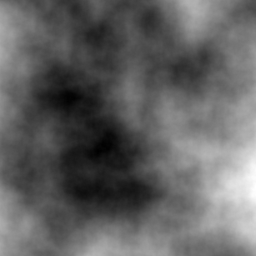
\includegraphics[width=0.35\linewidth]{images/background/generation/pnoise-8} \\
					\multicolumn{2}{r}{\tiny\textit{Perlin Noise Synthesis with 1, 2, 4 and 8 octaves}}
				\end{tabular}
			\end{column}
		\end{columns}
	\end{myframe}
	
	\section{Methodology}
	
	\subsection{Overview}
	
	\begin{myframe}[c]
		\begin{figure}
			\begin{center}
				\begin{tikzpicture}[
				font=\sffamily,
				every matrix/.style={column sep=0.5cm, row sep=0.5cm},
				phase/.style={draw, thick, align=center, fill=gray!35, inner sep=.6cm},
				to/.style={->,semithick,font=\sffamily\footnotesize},
				every node/.style={anchor=center}
				]
				
				\matrix[matrix of nodes,ampersand replacement=\&]
				{
					|[phase, text width = 2.5cm] (1)| \shortstack{CAD Modelling} \& 
					|[phase] (2)| \shortstack{Random Surface \\ Generation} \& 
					|[phase, text width = 2.5cm] (3)| \shortstack{Blending} \\
				};
				
				\draw[to] (1) -- (2);
				\draw[to] (2) -- (3);
				\end{tikzpicture}
			\end{center}
			
			\scriptsize\textit{Process Phases}
			\label{fig:process_phases}
		\end{figure}
	\end{myframe}
	
	\subsection{CAD Modelling}
	
	\begin{myframe}
		\centering
		\vspace{0.5em}
		\begin{tabular}{rl}
			
\includegraphics[width=0.3\linewidth]{images/methodology/base} &	
			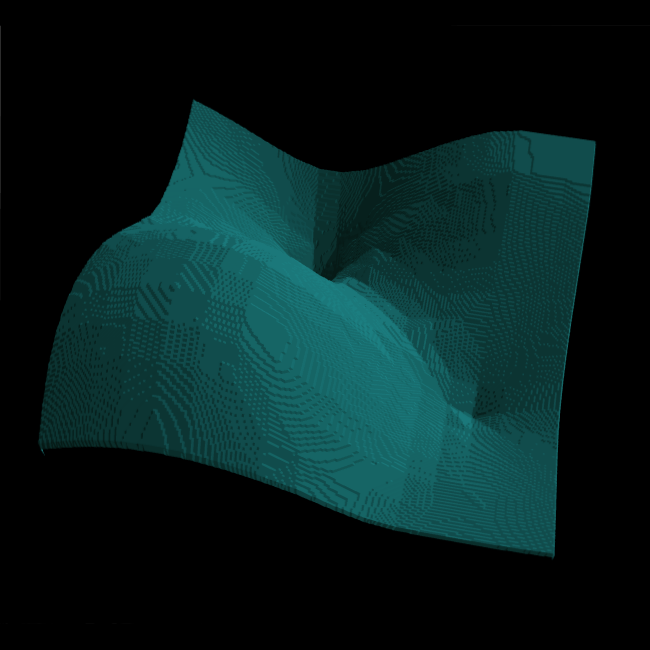
\includegraphics[width=0.3\linewidth]{images/methodology/base3d} \\
			\multicolumn{2}{c}{\scriptsize\textit{Example output from CAD Modelling Phase}}		
		\end{tabular}
	\end{myframe}
	
	\subsection{Random Surface Generation - Fourier Filtering}
	
	\begin{myframe}
	  \begin{figure}[!h]
    	\begin{center}
    		\begin{tikzpicture}[
    		font=\sffamily,
    		every matrix/.style={column sep=0.005cm, row sep=0.25cm},
    		every node/.style={anchor=center, font=\footnotesize, inner sep=.2cm},
    		source/.style={draw, thick, rounded corners, fill={rgb:red,1;green,2;blue,3}, text=white},
    		process/.style={draw, thick, fill=gray!35},
    		to/.style={->,semithick,font=\sffamily\footnotesize}
    		]
    		
    		\matrix[matrix of nodes, ampersand replacement=\&]
    		{
    			|[source] (1)| \shortstack{White noise  \\ matrix} \\
    			\& |[process] (2)| \shortstack{Fourier Transform} \\
    			\& \& |[process] (3)| \shortstack{$f^{-\beta}$ Filter} \\ 
    			\& \& \& |[process] (4)| \shortstack{Inverse \\ Fourier Transform} \\
    			\& \& \& \& |[source] (5)| \shortstack{Random Surface} \\
    		};
    		
    		\draw[to] (1) |- (2);
    		\draw[to] (2) |- (3);
    		\draw[to] (3) |- (4);
    		\draw[to] (4) |- (5);
    		
    		\end{tikzpicture}
    	\end{center}
	  \end{figure}		
	\end{myframe}
	
	\subsection{Random Surface Generation - Noise Synthesis}
	
	\begin{myframe}
		\centering
		\vspace{-2em}
		\[
			\frac{\sum_{i = 0}^{O - 1} noise(x \times L^i + B, y \times L^i + B) \times P^i}{ \sum_{i = 0}^{O - 1} P^i}
		\] \\[1em]
		\normalsize{
			\begin{tabular}{p{0.5em}ll}
				$O$ & octaves & Number of frequencies \\
				$L$ & lacunarity & Gap between successive frequencies \\
				$P$ & persistence & Contribution gap between successive octaves \\
				$B$ & base & Frequency displacement \\
				& noise & Noise function (eg. Perlin or Simplex)
			\end{tabular}
		}  
	\end{myframe}
	
	\subsection{Blending Process}
	
	\begin{myframe}
		\vspace{-2em}
		\begin{figure}[t]
			\pgfdeclareimage[width=3em]{base}{images/methodology/blending/base.png}
			\pgfdeclareimage[width=3em]{base-norm}{images/methodology/blending/base-norm.png}
			\pgfdeclareimage[width=3em]{random}{images/methodology/blending/random.png}
			\pgfdeclareimage[width=3em]{random-blur}{images/methodology/blending/random-blur.png}
			\pgfdeclareimage[width=3em]{mapped-base}{images/methodology/blending/mapped.png}
			\pgfdeclareimage[width=3em]{details}{images/methodology/blending/random-details.png}
			\pgfdeclareimage[width=3em]{adjusted-details}{images/methodology/blending/adjusted-details.png}
			\pgfdeclareimage[width=3em]{final}{images/methodology/blending/result.png}
			
			
			\begin{tikzpicture}[
			font=\sffamily,
			every matrix/.style={column sep=1cm, row sep=1cm},
			every node/.style={anchor=mid, text centered, font=\footnotesize, inner sep=.4cm},
			process/.style={draw, thick, fill=gray!35},
			to/.style={->,semithick,font=\sffamily\footnotesize}
			]
			
			\matrix (table) [matrix of nodes, ampersand replacement=\&]
			{
				|[process] (base)| \shortstack{Base \\ Mapping} \& \& 
				|[process] (random)| \shortstack{Detail \\ Extraction} \\
				\& |[process] (combine)| \shortstack{Combine \\ Operation} \& \\
			};
			
			\draw[to] (base.south) |- (0,1.5) -- (0,1.5) -| (combine.north);
			\draw[to] (random.south) |- (0,1.5) -- (0,1.5) -| (combine.north);
			
			% ++(0,-.5) -- ++(0,-.5)
			
			\end{tikzpicture}
		\end{figure}	
	\end{myframe}
	
	\subsection{Blending Process - Base Mapping}
	
	\begin{myframe}[c]
		\vspace{-2em}
		\begin{figure}
			\pgfdeclareimage[width=8em]{base}{images/methodology/blending/base.png}
			\pgfdeclareimage[width=8em]{base-norm}{images/methodology/blending/base-norm.png}
			\pgfdeclareimage[width=8em]{mapped-base}{images/methodology/blending/mapped.png}
			
			
			\begin{tikzpicture}[
				font=\sffamily,
				every matrix/.style={column sep=2cm, row sep=0.0cm},
				every node/.style={anchor=center, font=\footnotesize},
				source/.style={thick, inner sep = 0cm},
				to/.style={->,semithick,font=\sffamily\footnotesize}
				]
				
				\matrix[matrix of nodes, ampersand replacement=\&]
				{
					|[source] (base)| \pgfuseimage{base}
					\& |[source] (norm-base)| \pgfuseimage{base-norm}
					\& |[source] (mapped-base)| \pgfuseimage{mapped-base} \\
				};
				
				\draw[to] (base) -- node[pos=0.5, above] {Normalize} (norm-base);
				\draw[to] (norm-base) -- node[pos=0.5, above] {\shortstack{Spline \\ Mapping}} (mapped-base);
			\end{tikzpicture}
		\end{figure}	
	\end{myframe}
	
	\subsection{Blending Process - Detail Extraction}
	
	\begin{myframe}[c]
		\vspace{-1em}
		\begin{figure}
			\pgfdeclareimage[width=5em]{random}{images/methodology/blending/random.png}
			\pgfdeclareimage[width=5em]{random-blur}{images/methodology/blending/random-blur.png}
			\pgfdeclareimage[width=5em]{random-details}{images/methodology/blending/random-details.png}
			
			
			\begin{tikzpicture}[
			font=\sffamily,
			every matrix/.style={column sep=1cm, row sep=1cm},
			every node/.style={anchor=center, font=\footnotesize},
			source/.style={thick, inner sep = 0cm},
			to/.style={->,semithick,font=\sffamily\footnotesize}
			]
			
			\matrix[matrix of nodes, ampersand replacement=\&]
			{
				|[source] (random)| \pgfuseimage{random}
				\& \& |[source] (random-blur)| \pgfuseimage{random-blur} \\
				\& |[source] (random-details)| \pgfuseimage{random-details} \& \\
			};
			
			\draw[to] (random) -- node[pos=0.5, above] {\shortstack{Gaussian Blur}} (random-blur);
			\draw[to] (random-blur.south) |- (0,-0.2) -- (0,-0.2) -| node[pos=0.5, above] {\shortstack{Subtraction}} (random-details.north);
			\draw[to] (random.south) |- (0,-0.2) -- (0,-0.2) -| (random-details.north);
			\end{tikzpicture}
		\end{figure}	
	\end{myframe}
	
		\subsection{Blending Process - Combine Operation}
		
		\begin{myframe}[c]
			\vspace{-1em}
			\begin{figure}
				\pgfdeclareimage[width=5em]{base}{images/methodology/blending/base.png}
				\pgfdeclareimage[width=5em]{mapped-base}{images/methodology/blending/mapped.png}
				\pgfdeclareimage[width=5em]{random-details}{images/methodology/blending/random-details.png}
				\pgfdeclareimage[width=5em]{adjusted-details}{images/methodology/blending/adjusted-details.png}
				\pgfdeclareimage[width=5em]{final}{images/methodology/blending/result.png}
				
				
				\begin{tikzpicture}[
				font=\sffamily,
				every matrix/.style={column sep=0.25cm, row sep=-0.5cm},
				every node/.style={anchor=center, font=\footnotesize},
				source/.style={thick, inner sep = 0cm},
				to/.style={->,semithick,font=\sffamily\footnotesize}
				]
				
				\matrix[matrix of nodes, ampersand replacement=\&]
				{
					|[source] (base)| \pgfuseimage{base} \& \& |[source] (mapped-base)| \pgfuseimage{mapped-base} \& \& |[source] (random-details)| \pgfuseimage{random-details} \\
					
					\& \& \& |[source] (adjusted-details)| \pgfuseimage{adjusted-details} \& \& \\
					\& |[source] (final)| \pgfuseimage{final} \\
				};
				
				\draw[to] (mapped-base) -| node[pos=0.5, above] {Multiply} (adjusted-details);
				\draw[to] (random-details) -| node[pos=0.5, above] {Multiply} (adjusted-details);
				
				\draw[to] (base.south) |- (-4,0) -- (-4,0) -| node[pos=0.5, above] {Add} (final.north);
				\draw[to] (adjusted-details.west) -| (0,0) -- (0,0) -| (final.north);
				\end{tikzpicture}
			\end{figure}	
		\end{myframe}
	
	\section{Software}
	
	\subsection{Technologies}
	
	\begin{myframe}
		\vspace{-2em}
		\noindent
		\begin{columns}[t]
			\begin{column}{0.3 \linewidth}
				
\includegraphics[width=\linewidth]{images/technologies/angularjs}  \\[2em]
				\centering
				
\includegraphics[width=0.25\linewidth]{images/technologies/html5} \hspace{0.12\linewidth}
				
\includegraphics[width=0.25\linewidth]{images/technologies/es6} \hspace{0.12\linewidth}
				
\includegraphics[width=0.25\linewidth]{images/technologies/sass}
			\end{column}
			\begin{column}{0.3 \linewidth}
				
\includegraphics[width=0.70\linewidth]{images/technologies/babel} \hspace{0.75em}
				
\includegraphics[height=5em]{images/technologies/gulp} 				
				\\[2em]
				\centering
				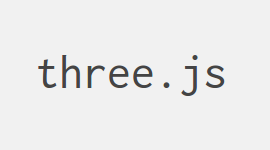
\includegraphics[width=0.85\linewidth]{images/technologies/threejs}
			\end{column}
			\begin{column}{0.3 \linewidth}
				
\includegraphics[width=\linewidth]{images/technologies/jspm}		  \\[2em]
				
\includegraphics[width=\linewidth]{images/technologies/webgl}
			\end{column}
		\end{columns}
	\end{myframe}
	
	\subsection{GPU Computations}
	
	\begin{myframe}
		\begin{columns}[T]
			\begin{column}{0.47\textwidth}
				\begin{block}{Technical Details}
					\begin{itemize}
						\item WebGL 2
						\item Render to Texture
						\item Floating-point textures
					\end{itemize}
				\end{block}
			\end{column}		
			\begin{column}{0.47\textwidth}
				\begin{block}{Features}
					
					\begin{itemize}
						\item FFT and IFFT
						\item Element-wise operations
						\item Matrix Normalization
					\end{itemize}
				\end{block}
			\end{column}	
		\end{columns}
	\end{myframe}
	
	\section{Demonstration}
	
	\begin{myframe}
		\vspace{-0.75cm}
		\centering
		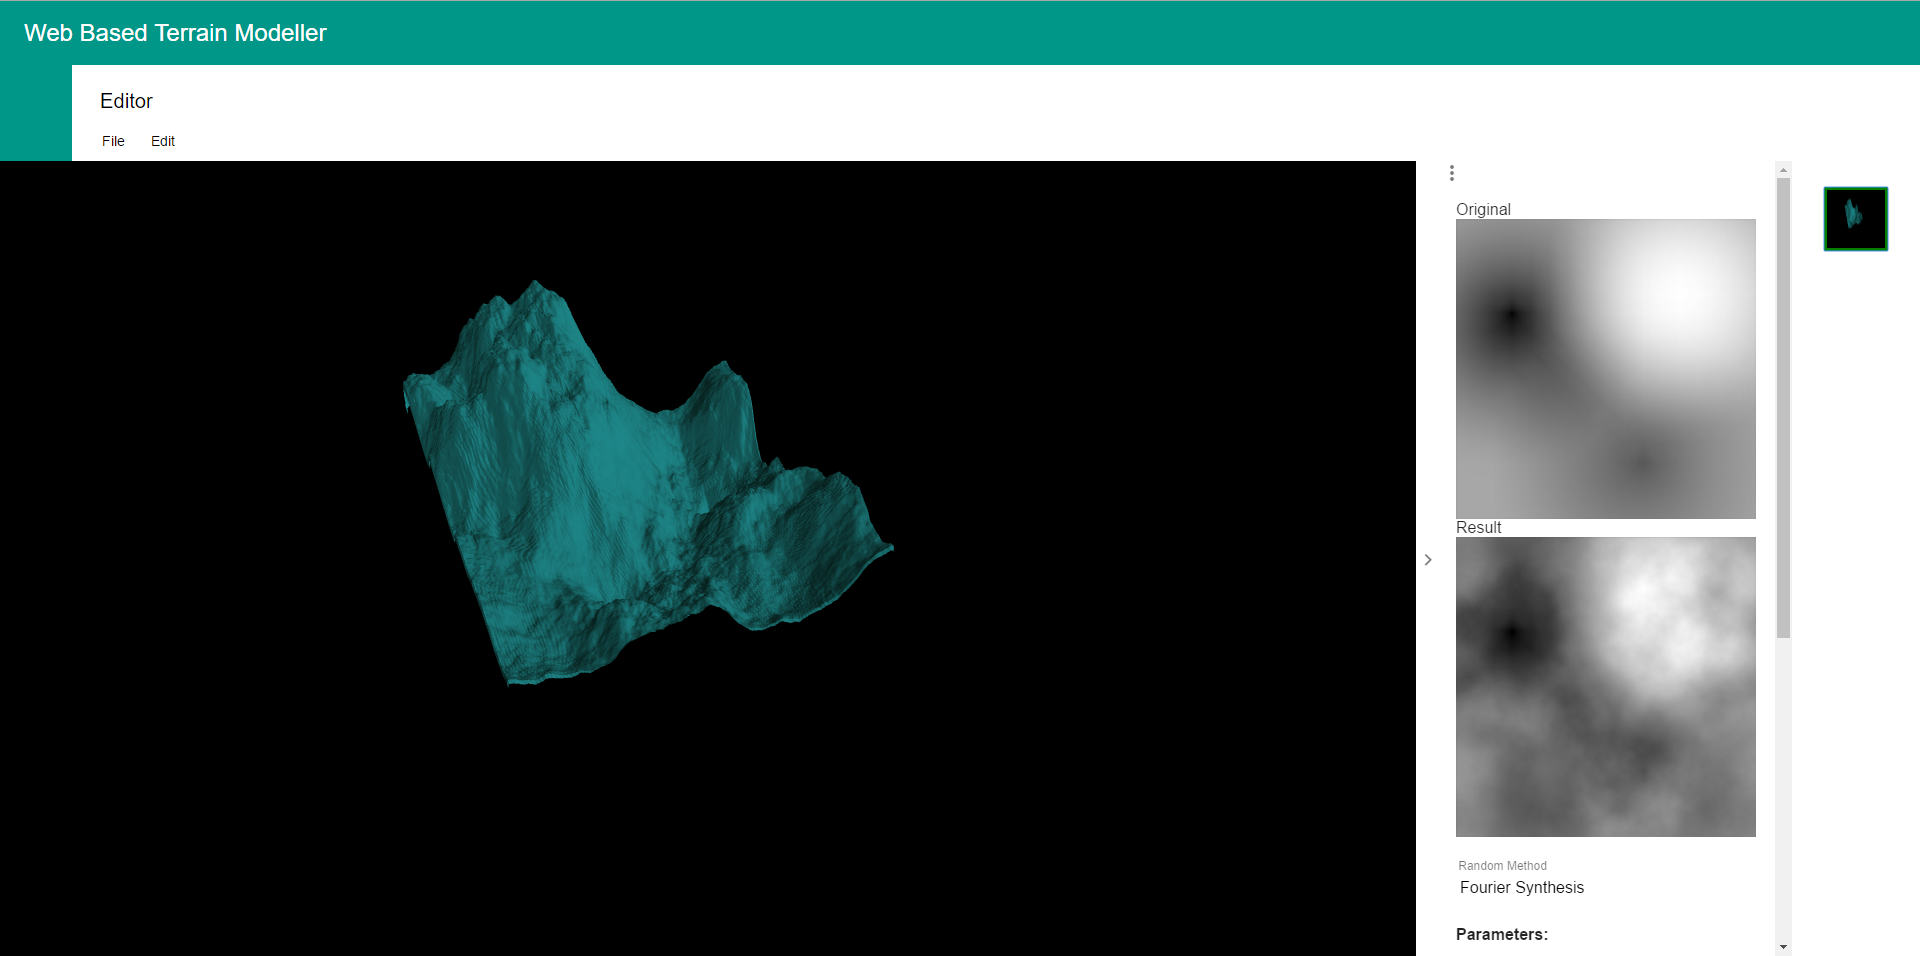
\includegraphics[width=0.9\linewidth]{images/results/demonstration}
	\end{myframe}
	
	\section{Benchmarks}
	
	%\subsection{Benchmarks}
	
%	\begin{myframe}[c]
%		\vspace{-0.75cm}
%		\centering
%		\begin{tabular}{ccc}
%			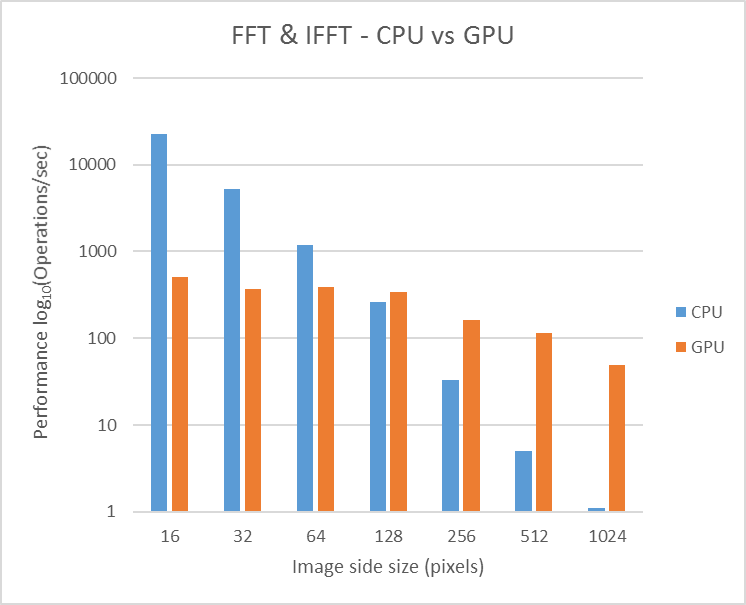
\includegraphics[width=0.3\linewidth]{images/results/benchmarks/plot-fft} &
%			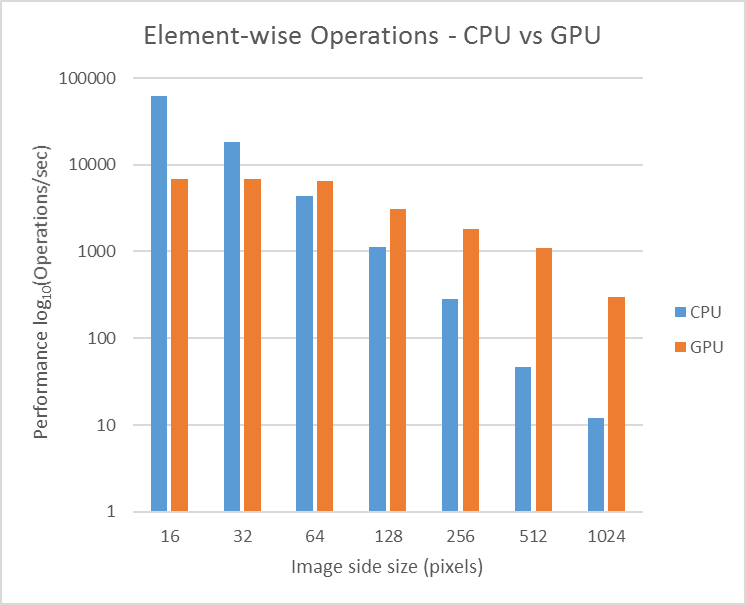
\includegraphics[width=0.3\linewidth]{images/results/benchmarks/plot-ewops} &
%			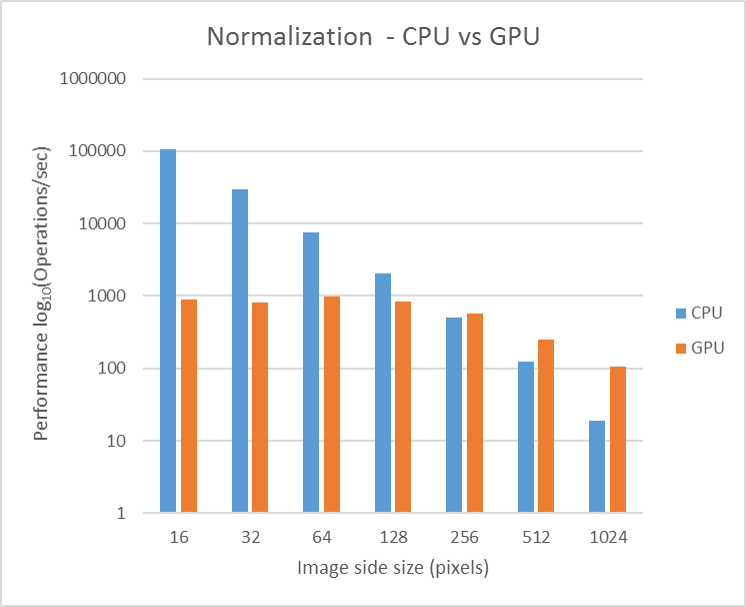
\includegraphics[width=0.3\linewidth]{images/results/benchmarks/plot-normalization} \\
%		\end{tabular}
%	\end{myframe}
%	
	\begin{myframe}[c]
		\vspace{-0.75cm}
		\centering
		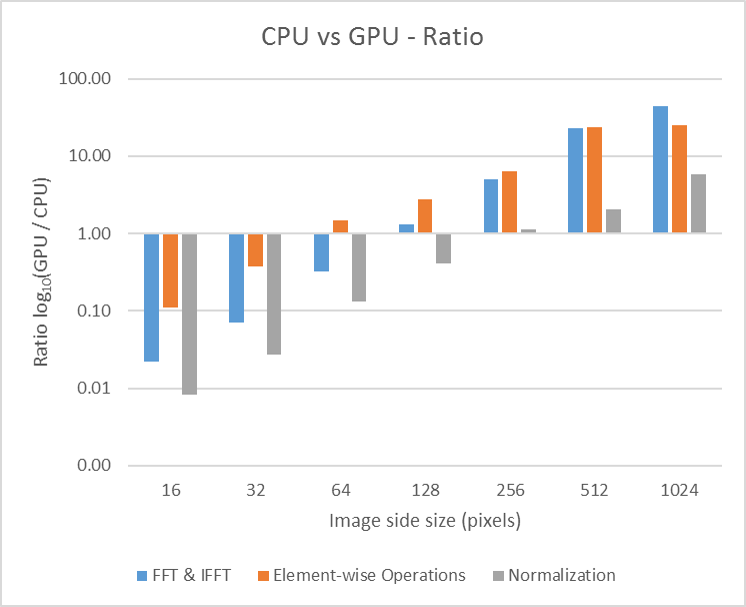
\includegraphics[width=0.55\linewidth]{images/results/benchmarks/plot-ratios}
	\end{myframe}
	
	\section{Conclusion \& Further Work}
	
	\begin{myframe}
		\vspace{-0.5cm}
		\begin{block}{What has been done}
			\begin{itemize}
				\item Hybrid Process for terrain modelling
				\item Web-based implementation
				\item WebGL 2 used for computations
			\end{itemize}
		\end{block}
		
		\begin{block}{Future Work}
			\begin{itemize}
				\item Different detail extraction methods
				\item Real world data
			\end{itemize}
		\end{block}
	\end{myframe}
\end{document}